\documentclass[a4paper, 12pt]{article}
\usepackage[utf8]{inputenc}
\renewcommand\familydefault{\sfdefault}
\usepackage[T1]{fontenc}
\usepackage[francais]{babel}
\usepackage[left=2cm,top=2cm,right=2cm,bottom=2cm]{geometry}
\usepackage{graphicx}
\usepackage{minted}
\usemintedstyle{colorful}
\usepackage{float}
\floatplacement{figure}{H}
\usepackage{authblk}
\usepackage{enumitem}
\usepackage{hyperref}
\hypersetup{
    colorlinks,
    citecolor=black,
    filecolor=black,
    linkcolor=black,
    urlcolor=blue
}

\usepackage{caption}
\newenvironment{code}{\captionsetup{type=listing}}{}

\begin{document}

\title{YourQuiz - Projet Logiciel}
\author{Raed Abdennadher, Mayron Bouchet, Matthieu Constant, \\ Nicolas Denby, Nathanael Nüfer, Steven Liatti}
\affil{\small Projet Logiciel - Profs. Yassine Rekik, Stéphane Malandain, Nabil Abdennadher}
\affil{\small Hepia ITI 3\up{ème} année}
\maketitle

\begin{figure}
	\begin{center}
		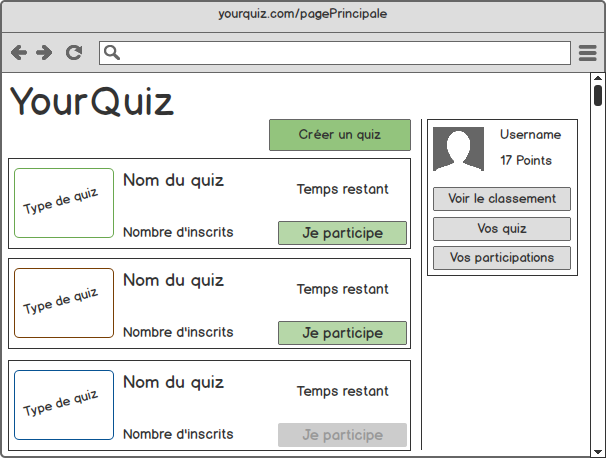
\includegraphics[width=0.85\textwidth]{../mockups/png/mainPage.png}
	\end{center}
\end{figure}
\newpage

\tableofcontents
\listoffigures
% \renewcommand\listoflistingscaption{Table des scripts de code}
% \listoflistings

\newpage

\section{Analyse}
\subsection{Définition des rôles}
\subsubsection{Utilisateur anonyme}
\begin{itemize}
    \item Inscription
    \item Connexion
    \item Visualiser les quiz disponibles
\end{itemize}
\subsubsection{Utilisateur connecté}
\begin{itemize}
    \item Créer un quiz
    \item S'inscrire à un quiz
    \item Participer à un quiz
    \item Supprimer un quiz (définir dans quelles conditions)
    \item Visualiser le classement
\end{itemize}
\subsection{Définition des besoins}
\subsubsection{Exigences du projet}
\begin{itemize}
    \item Définir des règles
    \item Les rôles des utilisateurs
    \item Réalisation d'un client Web et Mobile
    \item Déploiement Cloud
    \item Effectuer une montée en charge
    \item Mettre en place des tests de performance
\end{itemize}
\subsubsection{Exigences fonctionnelles}
Les fonctions et les services offerts par le logiciel :
\begin{itemize}
    \item Sign In
    \item Login
    \item Logout
    \item Création d'un quiz
    \item Inscription à un ou plusieurs quiz
    \item Participer à un quiz
    \item Voir la liste des quiz
\end{itemize}
\subsubsection{Exigences fonctionnelles}
\begin{itemize}
    \item Disponibilité
    \item Performance (gérer un grand nombre d'utilisateurs)
\end{itemize}

\section{Règles de fonctionnement du site}
\subsection{Participation}
Un quiz commence à un instant t. L'utilisateur peut commencer à répondre (démarrer) au quiz jusqu'à l'instant u (défini par le créateur). Par exemple : un quiz est ouvert de 12h à 18h. Les joueurs peuvent le commencer jusqu'à 17h59.
\bigbreak
La structure des questions est la suivante : pour une question, il y aura 4 réponses possibles et une seule bonne réponse. Une limite maximale de temps par question est définie. Cependant, une limite minimale et maximale seront définies par défaut (par exemple: min = 3 sec, max = 60 sec). Chaque question peut avoir un temps maximum différent.
\bigbreak
L'utilisateur est obligé de répondre à la question pour pouvoir continuer. Si l'utilisateur n'a pas répondu à la question avant la fin du temps imparti la réponse est considérée comme fausse et il passe automatiquement à la question suivante. Lorsqu'il répond à la question, on lui indique s'il a correctement répondu et on passe à la question suivante. L'utilisateur ne peut pas revenir en arrière. Il peut voir son score en tout temps et son avancement dans le questionnaire.
\bigbreak
Un système de coefficient multiplicateur par bonne réponse est présent. Au fur et à mesure que l'utilisateur répond juste aux questions, un coeffcient augmente jusqu'à une réponse fausse qui remet ce coefficient bonus à 0.
\bigbreak
Un questionnaire ne peut pas être refait. À la fin du quiz, on obtient un résumé de notre participation (bonnes/mauvaises réponses, score) et une note et des commentaires peuvent être donnés. Un système de ranking des quiz et créateurs de quiz sera mis en place.
\subsection{Création}
N'importe quel utilisateur peut créer un quiz, mais il ne peut pas participer à ses propres quiz. L'utilisateur choisi le nom, la description, le thème, le nombre de questions et les réponses possibles. Les utilisateurs peuvent signaler les quiz à contenu inapproprié. Si un certain nombre de clients signalent le quiz, une notification est envoyée aux administrateurs.
\bigbreak
Un quiz populaire pourrait avoir la possibilité d'être relancé après un certain temps. Une fois que le quiz est publié, son créateur ne peut ni le modifier ni le supprimer et les joueurs peuvent y participer. Une fois la période de jeu terminée, le créateur du quiz peut à nouveau modifier/supprimer le quiz.
\subsection{Consultation et recherche d'un quiz}
Les joueurs peuvent chercher les quiz par créateur, thème (tags). Il peuvent lire la description du quiz.

\newpage
\section{User stories}
\subsection{Utilisateur anonyme}
\begin{itemize}
    \item En tant qu’utilisateur anonyme, je veux pouvoir consulter les informations des quiz actuels.
    \item En tant qu’utilisateur anonyme, je veux pouvoir consulter le classement général de YourQuiz.
    \item En tant qu’utilisateur anonyme, je veux pouvoir m’inscrire au site YourQuiz.
\end{itemize}
\subsection{Utilisateur authentifié}
\begin{itemize}
    \item En tant qu’utilisateur non-authentifié, je veux pouvoir m’authentifier sur le site YourQuiz, afin d’avoir accès à son contenu.
    \item En tant qu’utilisateur authentifié, je veux pouvoir afficher/modifier mon profil personnel.
    \item En tant qu’utilisateur authentifié, je veux pouvoir avoir accès à la navigation du site YourQuiz.
    \item En tant qu’utilisateur authentifié, je veux pouvoir m’inscrire à un quiz d’un autre membre ayant encore de la place, afin de pouvoir y participer.
    \item En tant qu’utilisateur authentifié, je veux pouvoir participer à un quiz auquel je me suis inscrire lorsque la période pour effectuer le quiz est valide.
    \item En tant qu’utilisateur authentifié, je veux pouvoir consulter mes résultats par rapport à un quiz auquel j’ai participé.
    \item En tant qu’utilisateur authentifié, je veux pouvoir consulter ma place dans le classement générale, ainsi que les X meilleurs participants.
    \item En tant qu’utilisateur authentifié, je veux pouvoir consulter ma place dans le classement, selon une catégorie de mon choix, ainsi que les X meilleurs participants de cette catégorie.
    \item En tant qu’utilisateur authentifié, je veux pouvoir créer un quiz.
    \item En tant qu’utilisateur authentifié, je veux pouvoir visualiser le nombre de quiz que j’ai créé.
    \item En tant qu’utilisateur authentifié, je veux pouvoir publier, modifier ou supprimer mes quiz.
    \item En tant qu’utilisateur authentifié, je veux pouvoir relancer mes quiz qui sont terminés.
    \item En tant qu’utilisateur authentifié, je veux pouvoir signaler un quiz dont le contenu me paraît inapproprié, incomplet, ou ayant un problème autre.
    \item En tant qu’utilisateur authentifié, je veux pouvoir me déconnecter de mon compte YourQuiz.
\end{itemize}
\subsection{Administrateur}
\textit{Un administrateur possède les mêmes users stories qu’un utilisateur authentifié, ainsi que les cas suivants :}
\begin{itemize}
    \item En tant qu’administrateur authentifié, je veux pouvoir recevoir un message m’informant qu’un quiz a été signalé X fois, afin de prendre les mesures nécessaires.
    \item En tant qu’administrateur authentifié, je veux pouvoir avoir accès à l’ensemble des quiz des utilisateurs, afin de supprimer ceux qui me seraient signalé.
\end{itemize}

\section{Modélisation}
\begin{figure}
	\begin{center}
		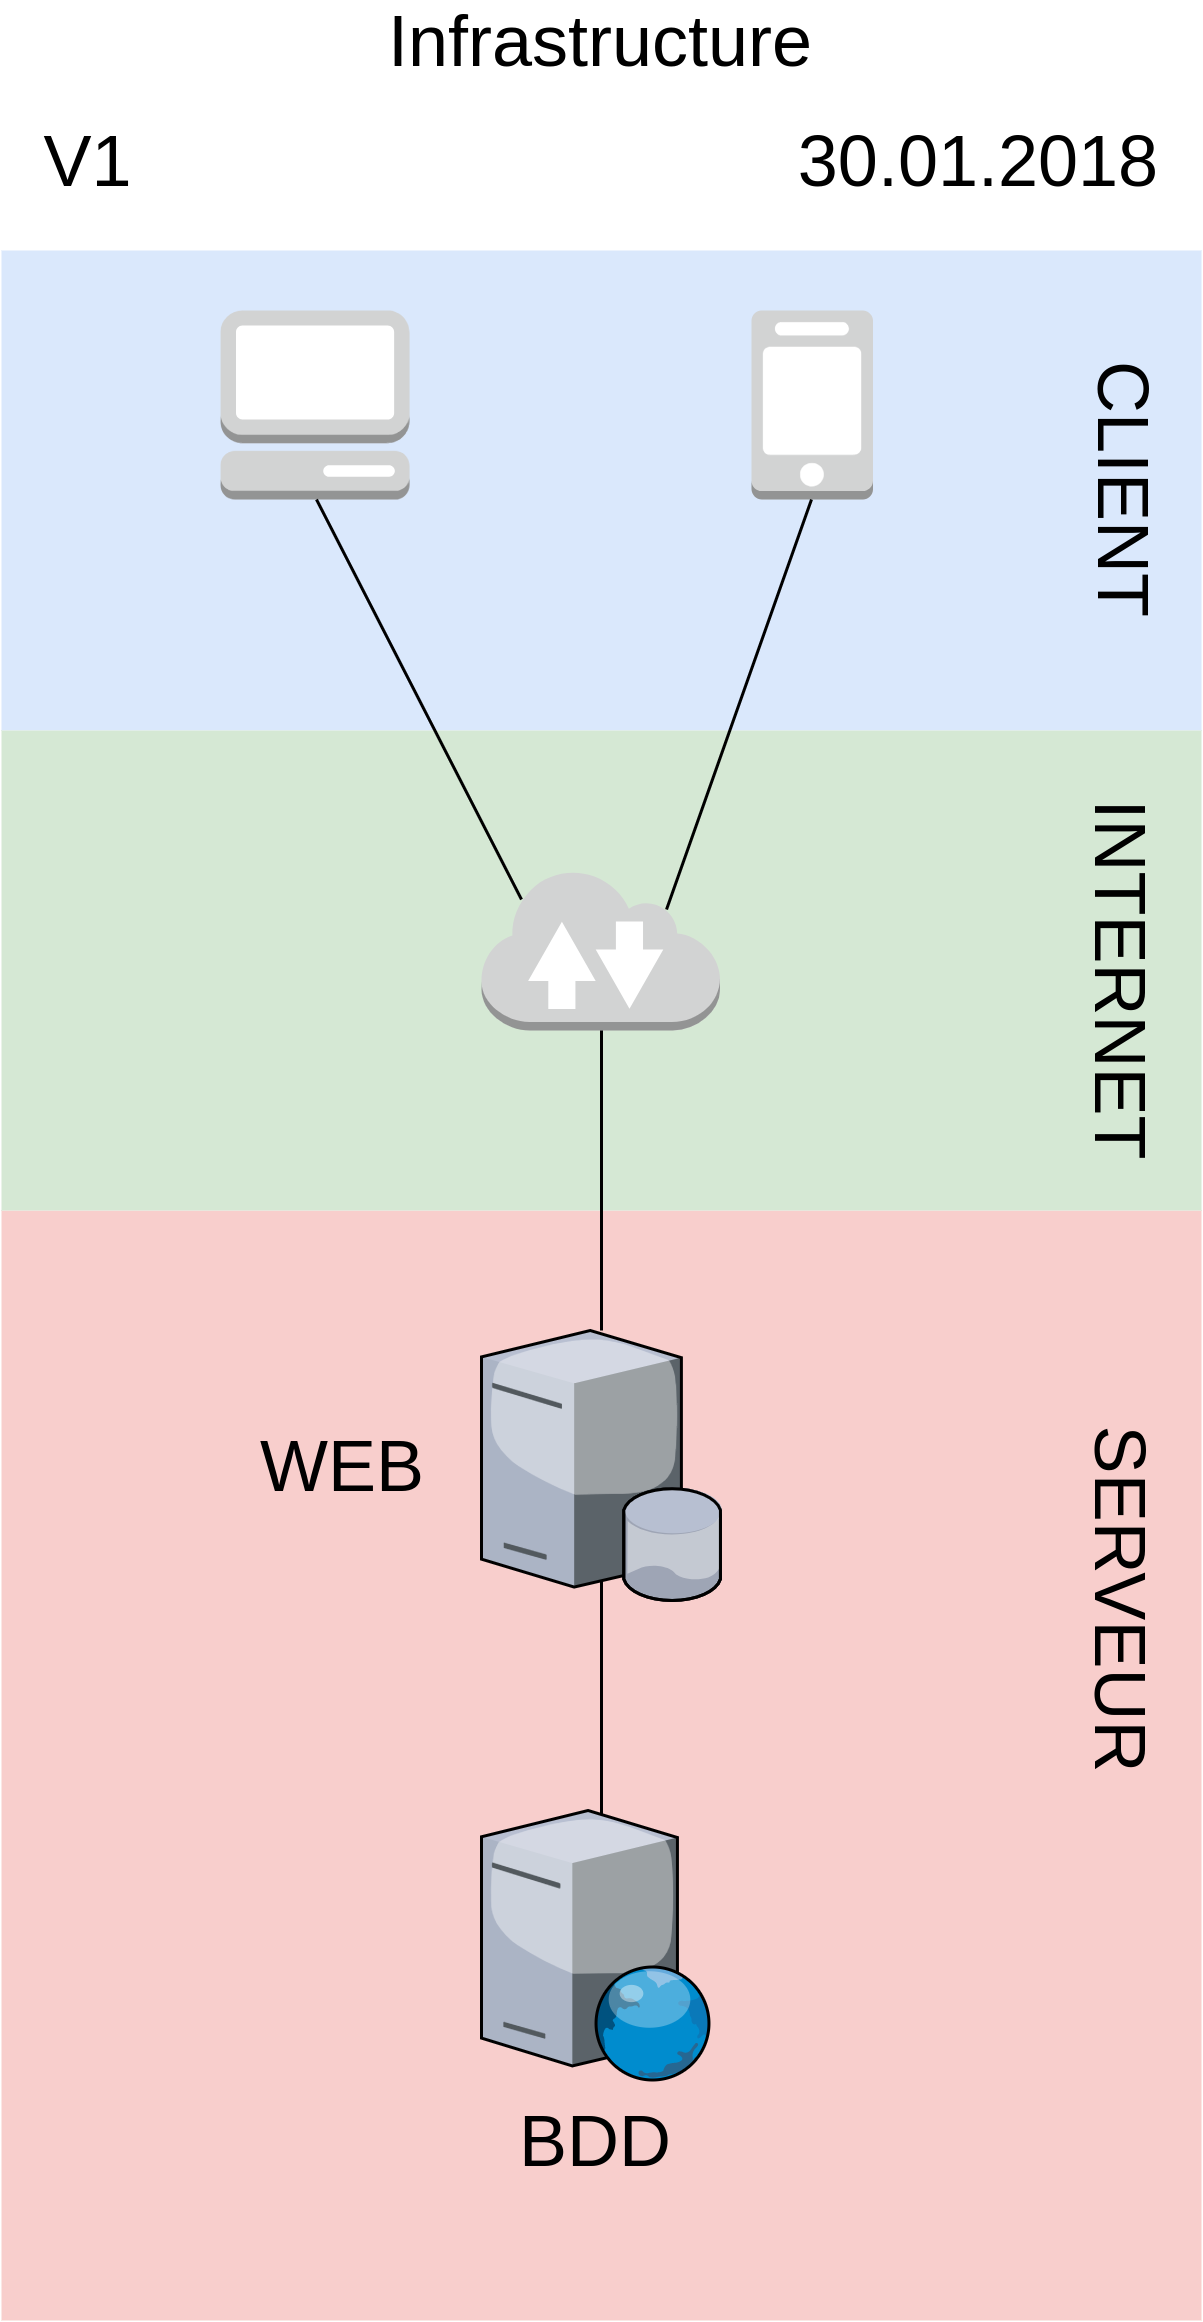
\includegraphics[width=0.5\textwidth]{../diagrams/infrastructure.png}
	\end{center}
    \caption{Infrastructure}
\end{figure}
\subsection{Diagrammes d’activités}
\subsubsection{Login}
\begin{figure}
	\begin{center}
		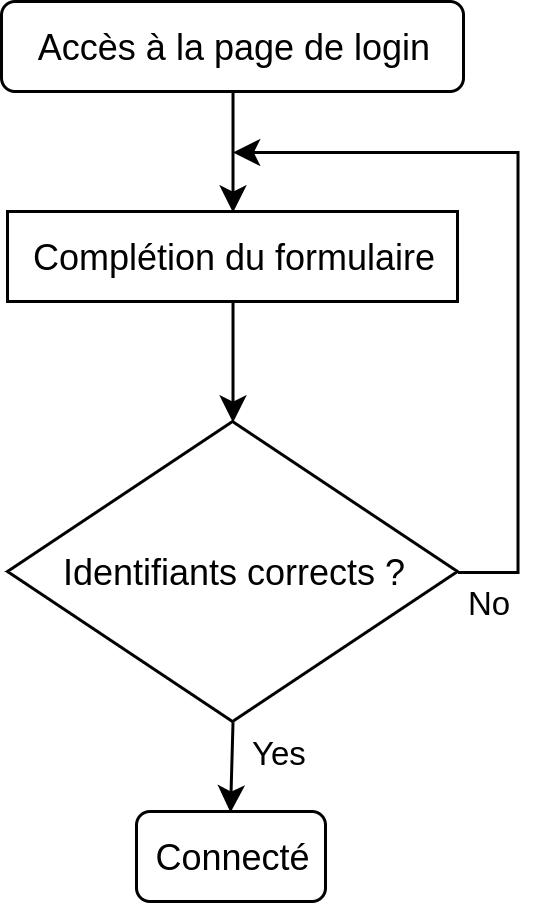
\includegraphics[width=0.5\textwidth]{../diagrams/login.png}
	\end{center}
    \caption{Login}
\end{figure}
\subsection{Diagramme d'utilisation}
\begin{figure}
	\begin{center}
		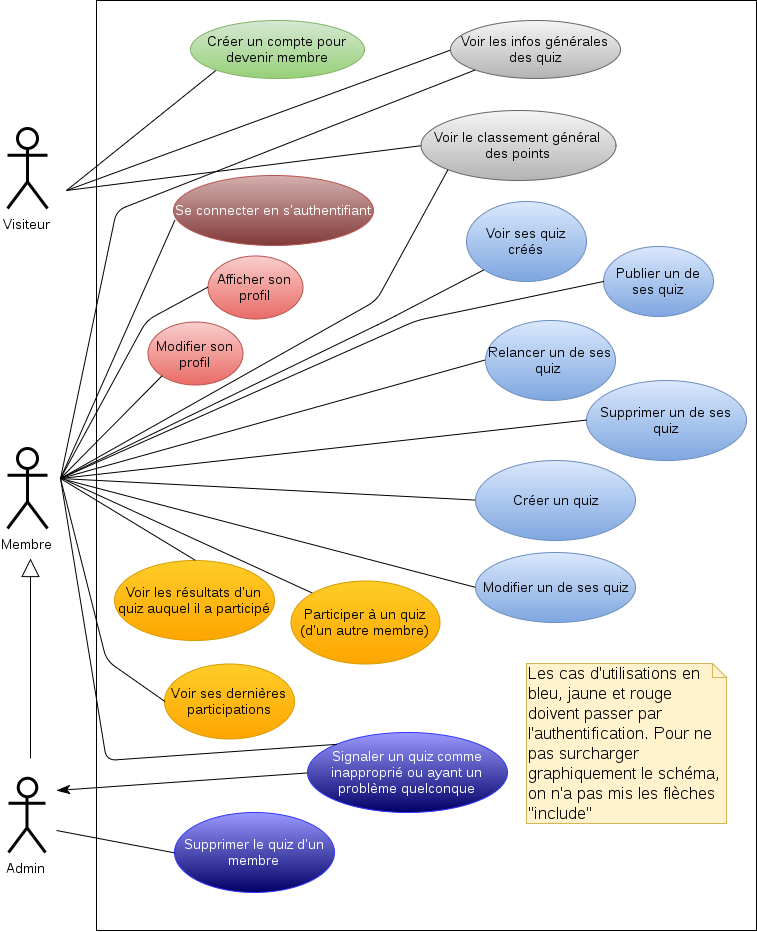
\includegraphics[width=1.0\textwidth]{../diagrams/UseCaseQuiz.png}
	\end{center}
    \caption{Use case}
\end{figure}

\subsection{Maquettes}
\begin{figure}
	\begin{center}
		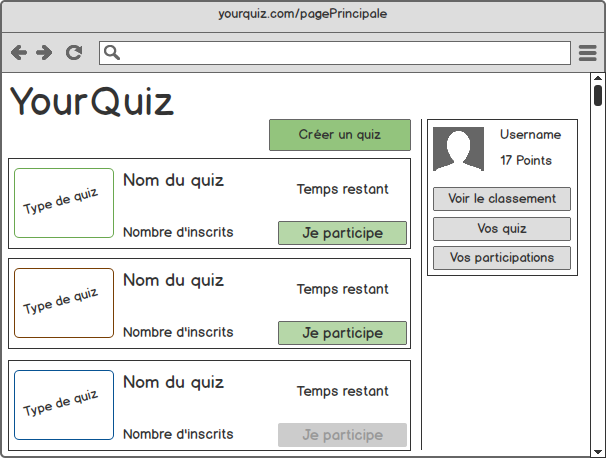
\includegraphics[width=0.73\textwidth]{../mockups/png/mainPage.png}
        \caption{mainPage}
	\end{center}
\end{figure}
\begin{figure}
	\begin{center}
		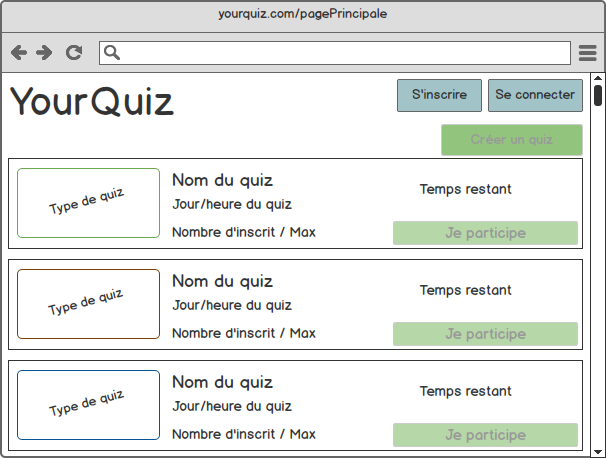
\includegraphics[width=0.73\textwidth]{../mockups/png/notMemberHome.png}
        \caption{notMemberHome}
	\end{center}
\end{figure}
\begin{figure}
	\begin{center}
		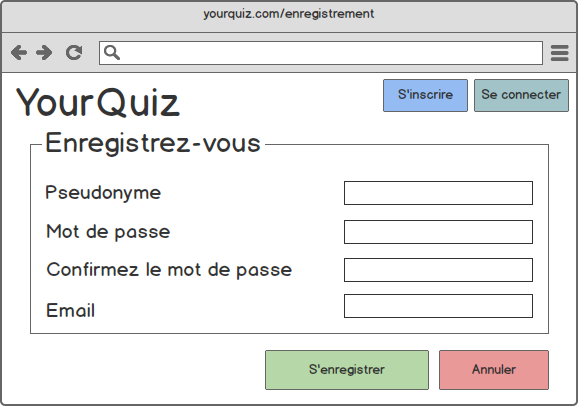
\includegraphics[width=0.73\textwidth]{../mockups/png/enregistrement.png}
        \caption{enregistrement}
	\end{center}
\end{figure}
\begin{figure}
	\begin{center}
		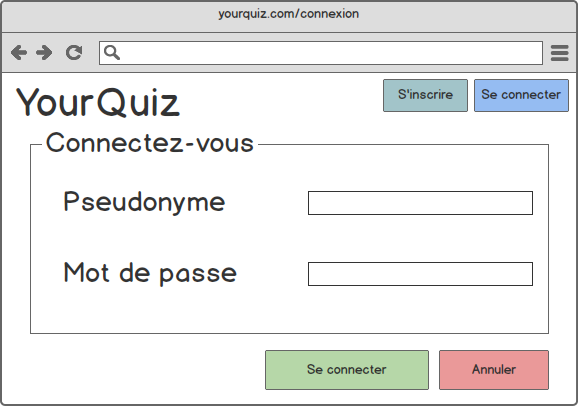
\includegraphics[width=0.73\textwidth]{../mockups/png/logIn.png}
        \caption{logIn}
	\end{center}
\end{figure}
\begin{figure}
	\begin{center}
		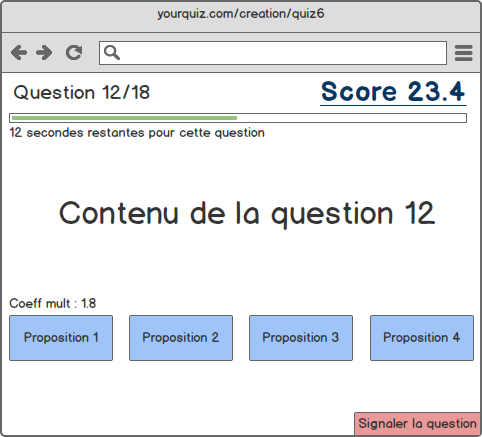
\includegraphics[width=0.73\textwidth]{../mockups/png/inQuestion.png}
        \caption{inQuestion}
	\end{center}
\end{figure}
\begin{figure}
	\begin{center}
		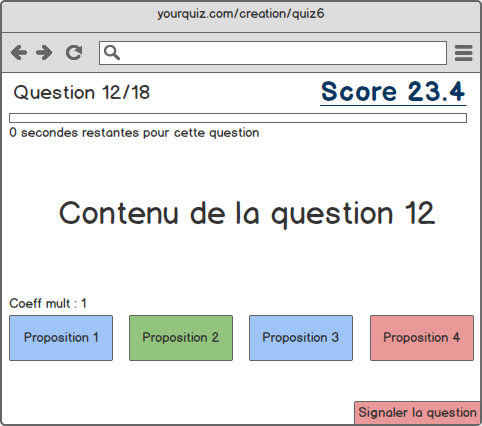
\includegraphics[width=0.73\textwidth]{../mockups/png/afterQuestion.png}
        \caption{afterQuestion}
	\end{center}
\end{figure}
\begin{figure}
	\begin{center}
		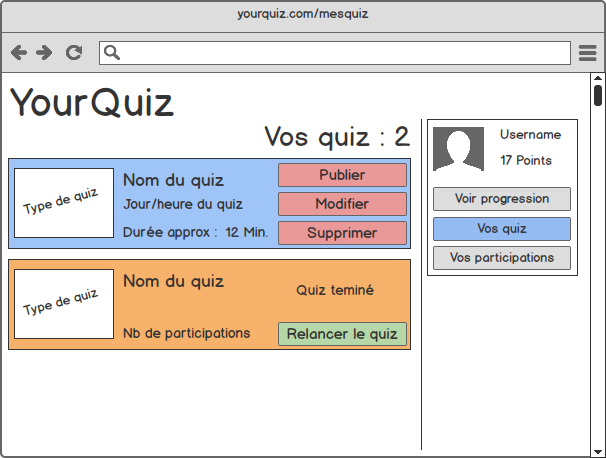
\includegraphics[width=0.73\textwidth]{../mockups/png/myQuiz.png}
        \caption{myQuiz}
	\end{center}
\end{figure}
\begin{figure}
	\begin{center}
		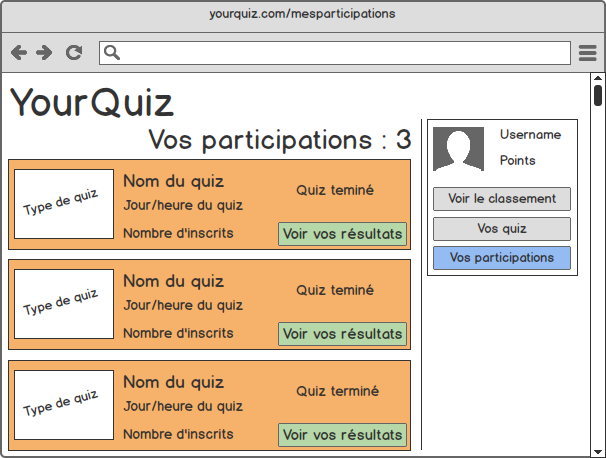
\includegraphics[width=0.73\textwidth]{../mockups/png/myParticipations.png}
        \caption{myParticipations}
	\end{center}
\end{figure}
\begin{figure}
	\begin{center}
		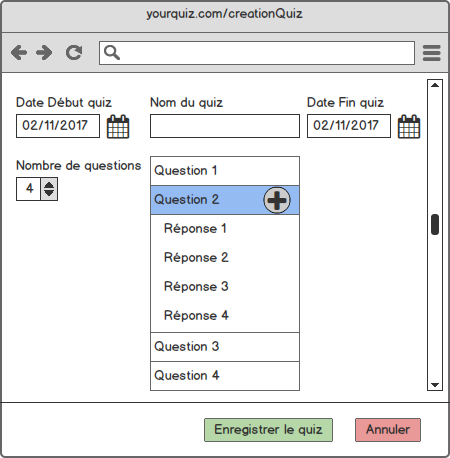
\includegraphics[width=0.73\textwidth]{../mockups/png/createQuiz.png}
        \caption{createQuiz}
	\end{center}
\end{figure}
\begin{figure}
	\begin{center}
		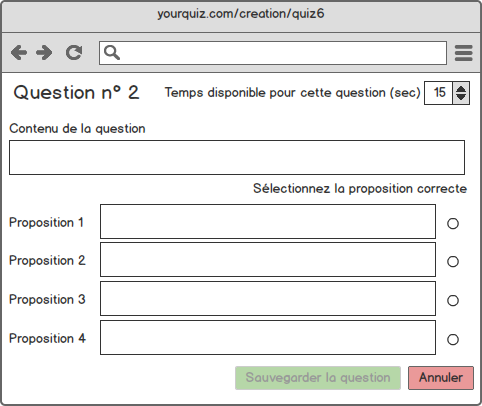
\includegraphics[width=0.73\textwidth]{../mockups/png/createQuestion.png}
        \caption{createQuestion}
	\end{center}
\end{figure}
\begin{figure}
	\begin{center}
		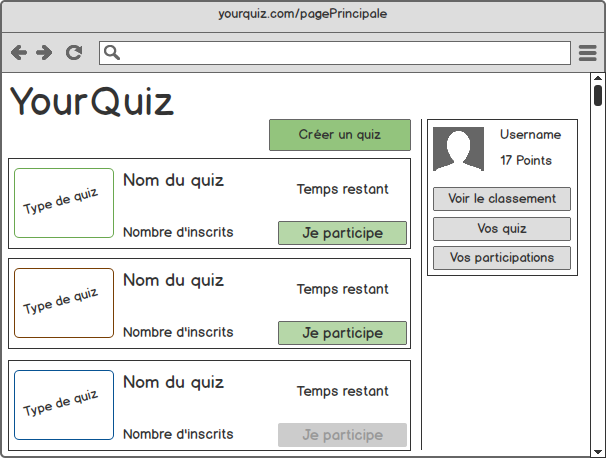
\includegraphics[width=0.73\textwidth]{../mockups/png/mainPage.png}
        \caption{mainPage}
	\end{center}
\end{figure}


% \begin{code}
%     \inputminted[breaklines,breaksymbol=,linenos,frame=single,stepnumber=1,tabsize=2]{language}{code}
%     \caption{Légende}
%     \label{my_ref}
% \end{code}

% \href{https://www.vagrantup.com/}{Vagrant}

% \mintinline{text}{root}


\end{document}
